\chapter*{Preface}
\addcontentsline{toc}{chapter}{Preface}

This Master’s Thesis is written by Andrej Orsula as his final work of M.Sc. programme in Robotics at Aalborg University during the academic year 2020/21.


\section*{Acknowledgements}

Special thanks goes to Simon Bøgh for his supervision, guidance and numerous discussions throughout the whole process that helped shaping this project.
Moreover, I must express a very profound gratitude to my mum, dad, sister and brother for their love and everlasting support.


\section*{Additional Resources}

\noindent
<TODO: YouTube playlist>.
\begin{itemize}
    \item[{
\includegraphics[height=8pt]{_misc/youtube_logo.pdf}}] \href{https://youtube.com/playlist?list=PLzcIGFRbGF3Qr4XSzAjNwOMPaeDn5J6i1}{https://youtube.com/playlist?list=PLzcIGFRbGF3Qr4XSzAjNwOMPaeDn5J6i1}
\end{itemize}

\noindent
The source code developed during this project is freely available on the following \textit{GitHub} repository.
\begin{itemize}
    \item[{
\includegraphics[height=8pt]{_misc/github_logo.pdf}}] \href{https://github.com/andrejorsula/drl_grasping}{https://github.com/andrejorsula/drl\_grasping}
\end{itemize}

\noindent
All readers interested in reproducing the results from this work are welcome to use pre-built \textit{Docker} images that can be pulled from \textit{Docker Hub}.
\begin{itemize}
    \item[{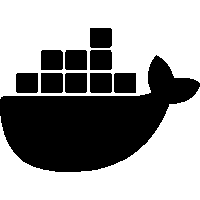
\includegraphics[height=8pt]{_misc/docker_logo.pdf}}] \href{https://hub.docker.com/r/andrejorsula/drl_grasping}{https://hub.docker.com/r/andrejorsula/drl\_grasping}
\end{itemize}

\noindent
This manuscript can be accessed on the following \textit{GitHub} repository, together with additional resources such as raw data collected during the experiments.
\begin{itemize}
    \item[{
\includegraphics[height=8pt]{_misc/github_logo.pdf}}] \href{https://github.com/andrejorsula/master_thesis}{https://github.com/andrejorsula/master\_thesis}
\end{itemize}
